\documentclass[a4paper,11pt]{article}
\usepackage[margin=2cm]{geometry}

\usepackage[titletoc,toc,title,page]{appendix}
\usepackage[nodayofweek]{datetime}
\usepackage{cite}
\usepackage{graphicx}
\longdate

\usepackage{minted}
\usepackage{titlesec}
\usepackage{hyperref}
\usepackage{fancyhdr}
\pagestyle{fancyplain}
\fancyhf{}
\lhead{\fancyplain{}{M.Sc.\ Group Project Report}}
\rhead{\fancyplain{}{\today}}
\cfoot{\fancyplain{}{\thepage}}


\title{Implementation of attentional bistability of the dragonfly visual neurons in an intelligent biomimetic agent\\\Large{--- Report Two ---}}
\author{Juan Carlos Farah, Panagiotis Almpouras, Ioannis Kasidakis, Erik Grabljevec, Christos Kaplanis\\
       \{jcf214, pa512, ik311, eg1114, ck2714\}@doc.ic.ac.uk\\ \\
       \small{Supervisors: Professor Murray Shanahan, Zafeirios Fountas, Pedro Mediano}\\
       \small{Course: CO530/533, Imperial College London}
}

\begin{document}
\maketitle
\section{Challenges and Motivation for New Specifications}
In this section, we motivate our change in specifications by highlighting the biggest challenges that we have encountered in our project. 

Our most significant challenge has been to generate the output we expect from the CSTMD1 (Central small target motion detector) neurons, given an input from the initial visual processing ESTMD (elementary small target motion detector) neurons. In part (iii) of Stage 1A, as specified in Report 1, we expected to observe evidence that the CSTMD1, when presented with two targets in the visual receptive field, will select one of them. However, the CSTMD1 model is not currently displaying this selectivity as shown in Figure 1. What we expected was that the firing rate graph for both targets would emulate that of one of the two. Instead, what we are observing is a CSTMD1 neuron that fires more frequently when both targets are present.

	\begin{figure}[h]
	\begin{center}
	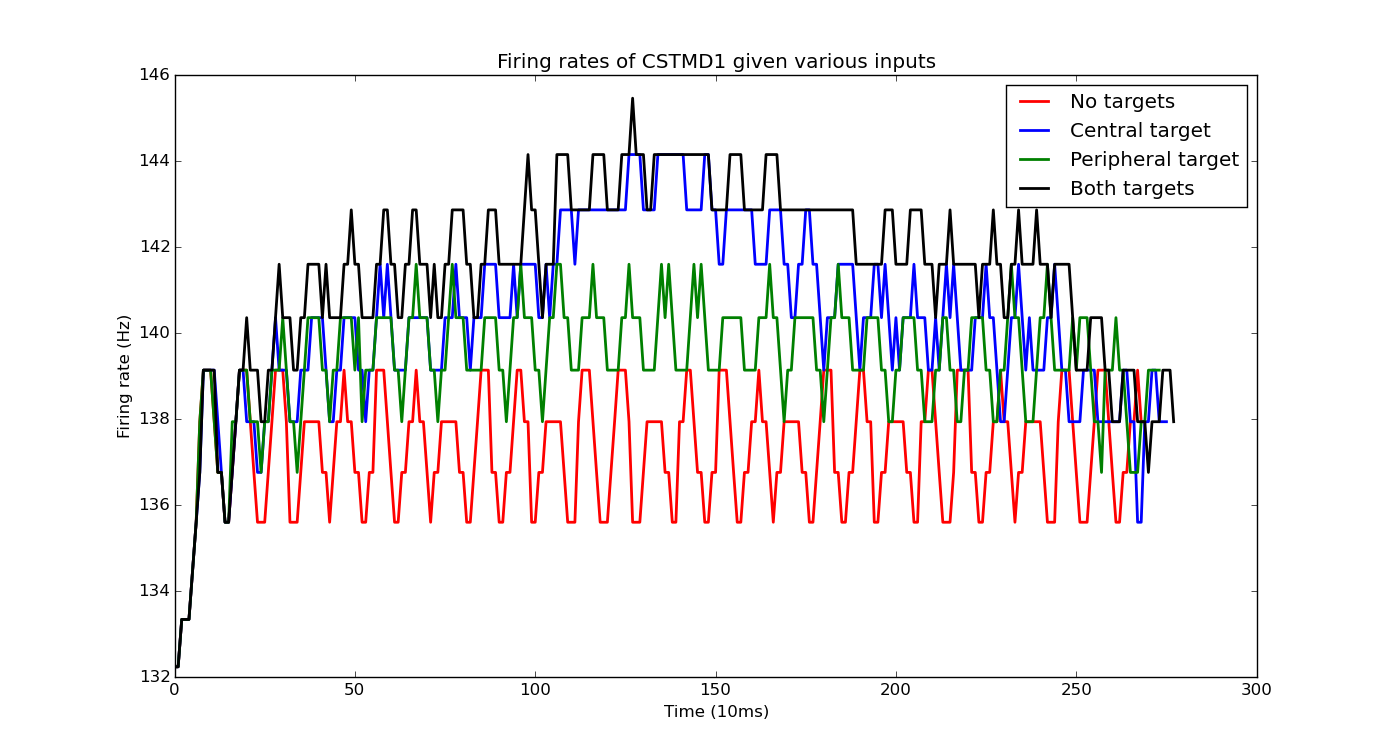
\includegraphics[scale = 0.3]{firingrates}
	\end{center}
	\caption{Firing rates of CSTMD1}
	\end{figure}	

Given the complicated nature of the morphologically-modelled CSTMD1, which is largely third party code, and the fact that this target selection has never been shown before in a CSTMD1 model, we are concerned that we may not be able to reproduce this phenomenon as shown by biological CSTMD1 neurons within the time constraints of this project. While it is still our goal to do so, we are moving this part of the specifications out of minimum requirements and into our possible extensions.

In light of this change, we have added a task to our specification consisting of designing a web client that will enable users to:
\begin{enumerate}
	\item Modify key parameters in each of the components of our dragonfly visual system model.
	\item Run each component individually and display key metrics demonstrating the functionality of each component.
	\item Run the components in unison and display key metrics demonstrating the functionality of the system as a whole.
\end{enumerate}
This would enable us, and external users, to efficiently investigate the properties of our dragonfly visual system and better tune the parameters in order to achieve target selection and prey capture with our model.

\section{New Specifications}
Below we layout our new requirements and the revised stage of completion for each part:
\begin{center}
    \begin{tabular}{p{12cm} c c}
    \textbf{Minimum Requirements (Stage 1)} & \textbf{Completion} \\ \hline
    (Ai) Create an animation tool to generate inputs for visual processing. & Full \\ 
	(Aii) Build a model for the ESTMD neuron present between the retina and the actual CSTMD1 neurons of a real dragonfly. & Full \\
	(Aiii) Design connection between ESTMD and CSTMD1 neurons. & Full \\
	(B) Build a layer of pattern recognition neurons that can learn to recognise spike patterns within a noisy background. & Full\\
	(C) Integrate the visual processing and pattern recognition system to detect patterns within the CSTMD1 output and add a simple action selection mechanism. & Partial\\
    \end{tabular}
\end{center}

\begin{center}
    \begin{tabular}{p{12cm} c c}
    \textbf{Expected Implementation (Stage 2)} & \textbf{Completion} \\ \hline
	(A) Develop a web client to analyse metrics of each component of our model. & Partial \\
	(B) Create a virtual 3D environment for the dragonfly agent. & None\\
	(C) Enhance the action selection mechanism to control the agent within the environment. & None\\
    \end{tabular}
\end{center}

\begin{center}
    \begin{tabular}{p{12cm} c c}
    \textbf{Possible Extensions (Stage 3)} & \textbf{Completion} \\ \hline
	(A) Achieve CSTMD1 target selection through experimentation with various parameters and connections with the ESTMD neurons. & Partial\\
	(B) Improve usability and features of web client. & None\\
	(C) Implement the agent in a quadcopter drone. & None\\
    \end{tabular}
\end{center}


\section{Progress}

\subsection{Animation Tool}
In order to generate input for our visual pre-processing layer, we developed an animation tool using Pyglet. This allows the user the option to create a video of black targets moving across a custom background that is either stationary or moving. The size and velocity vector of each target is adjustable.

\subsection{Visual Processing}
We successfully implemented a model for ESTMD (elementary small-target-motion detection) based on \cite{hal11}. The model can detect small-target motion across a moving, complicated background. This stage required research into spatio-temporal filters that approximate the function of real ESTMD neurons. The input of the ESTMD can either be a full video or frame by frame as it is produced by the animation tool. The output of the ESTMD model is a time series of matrices of processed pixels, which can be viewed in a video. This output is connected to the CSTMD1 neurons by converting each pixel into a firing rate for a simple integrate-and-fire neuron and connecting the output of each of these neurons to the CSTMDs. Sample screenshots of video input and output are included in Appendix A.

\subsection{Pattern Recognition}
To model the pattern recognition neurons, we initially replicated experiments conducted by T. Masquelier et al. \cite{stdp2} \cite{stdp1} . The resulting code was a Python module for Spike Response Model (SRM) leaky integrate-and-fire neurons that successfully recognised input patterns based on the samples described in the respective papers. A single of these neurons is able to successfully recognise a recurring pattern within background noise and a network of them is able to do so for multiple patterns. We then extended the module so that the neurons can be easily adapted to recognise input with varying properties such as average firing rate, number of afferents, frequency of pattern appearance, amongst others. This implementation is able to recognise patterns output from our CSTMD1 neurons and measures the effectiveness of the pattern recognition neurons by tracking key information such as true-positive, false-positive and true-negative spike incidences. Sample plots for this module are included in Appendix B.

\subsection{Web Client}
The web client is designed to be a simple interface through which simulations for each of the modules can be run and automated, both separately and jointly. We have currently implemented a prototype using Bottle and MongoDB and have connected it to the pattern recognition module. This graphical user interface provides the minimal functionality needed to create sample spike trains, test pattern recognition neurons against them and save the results of each experiment, providing key insight to the effect of each parameter on the output.


\section{Updated Task Schedule}	

Below is a condensed version of our updated schedule. Sprints are two weeks long, with Sprint 3 having started on 4 March 2015. Priorities are ranked 1 (highest) to 4 (lowest). 

\subsection{Stage 1C: CSTMD1 and Pattern Recognition Integration}
\begin{center}
    \begin{tabular}{p{12cm} c c}
    \textbf{Task} & \textbf{Priority} & \textbf{Sprint} \\ \hline
	Get pattern recognition to detect short patterns from CSTMD output. & 1 & 3-4 \\
	Layer pattern recognition neurons to recognise longer patterns. & 1 & 3-4\\
	Create simple action selection mechanism. & 1 & 4 \\
    \end{tabular}
\end{center}

\subsection{Stage 2: Web Client and Enhanced Action Selection}
\begin{center}
    \begin{tabular}{p{12cm} c c}
    \textbf{Task} & \textbf{Priority} & \textbf{Sprint} \\ \hline
    Define range of actions available to biomimetic agent. & 2 & 4 \\
    Design and implement basic environment for simulated agent. & 2 & 4-5 \\
    Implement adapted Braitenberg vehicle as action selection mechanism. & 2 & 4-5 \\
	Parametrise components of visual system for integration into web client. & 2 & 4 \\
	Integrate classes of components into web client. & 2 & 4-5 \\	
	Implement useful metrics for each component in web client. & 2 & 4-5 \\
    \end{tabular}
\end{center}

\subsection{Stage 3: Target Selection and Improved Web Client}
\begin{center}
    \begin{tabular}{p{12cm} c c}
    \textbf{Task} & \textbf{Priority} & \textbf{Sprint} \\ \hline
    Get CSTMD to select between targets. & 3 & 3-6 \\
    Implement agent in a quad-copter drone. & 4 & 6-7 \\
    \end{tabular}
\end{center}

\section{Testing}

\subsection{Methodology}
Our testing strategy has evolved from simple ``on the run manual testing'' to full systematic unit testing of our entire codebase. We followed our project's modular and class-based architecture while designing our testing structure. Each class has a corresponding test class, whose test methods aim to mirror the methods of the class it is testing. However, it is possible that several test methods cover different parts of the same method, or that in turn one test method covers several methods.

Following the white-box testing strategy, each test class is designed by the team members who wrote the original code and who therefore have the best insight regarding the expected behaviour of the original class. Currently we have focused our testing on covering as many branches as possible, each of which is analysed for the different possible behaviours it may have. We are measuring our code coverage by the percentage of statements covered. 

As we progress with our development we aim to augment our testing strategy to include component, integration and system tests. Component tests will cover end-to-end cases for each of our modules, while integration tests will cover the connections between each of these components. Finally, system tests will cover the complete project, when all modules have been connected between themselves and the web client.

\subsection{Implementation}
Given that all of our code is written in Python, we use Python's unittest framework. To measure code coverage we are using Python's coverage library, which allows us to run tests on each file separately and combine results to create comprehensive reports.

\subsection{Results}
Our current test coverage is 81\%. Details results from our latest test run covering all of our modules can be found in Appendix C.

\subsection{Challenges}
At this stage, some of the functionalities we are developing have not been factored out optimally, which causes some methods to be very tightly interlinked. This in turn requires more complex tests, some of which will need extensive modification as we restructure the code. We have thus decided to omit some of these methods from our current tests. As we gain more experience with unit testing and refine our design, these methods will be covered.

We also found it difficult to test the graphical output that our modules produce. While testing it manually is very straightforward, we encountered problems while writing tests to do so systematically. One solution we employed was to store images of the graphics and check the values of specific pixels against the expected ones, which we defined beforehand. This approach becomes more complicated when random elements are involved and when the result can vary. We currently handle this by setting specific seeds for the pseudorandom number generators and allowing some error in the test calculations. However, we are still working to make these tests more resilient.

\bibliography{report2}{}
\bibliographystyle{plain}

\newpage
\begin{appendices}
\section{Animation / ESTMD Sample Screenshots}
Below are screenshots of an animation of a small target moving diagonally across a moving complicated background (left) and a screenshot of the corresponding output of the ESTMD. Despite the moving background, the ESTMD highlights the small moving target. \\ \\

\includegraphics[scale = 0.4]{input}

\includegraphics[scale = 0.5]{processed}

\section{Pattern Recognition Sample Plots}
\subsection{Single Neuron / Single Pattern}
A single pattern recognition neuron is able to detect a recurring pattern (shown in gray) within a noisy background. At the beginning of the simulation, the neuron is not selective and fires repeatedly, as shown below on the left. However, spike-timing-dependent plasticity allows the neuron to become selective to the pattern and towards the last quarter of the simulation, fires consistently when it appears, as shown below on the right. \\

\begin{figure}[h]
\centering
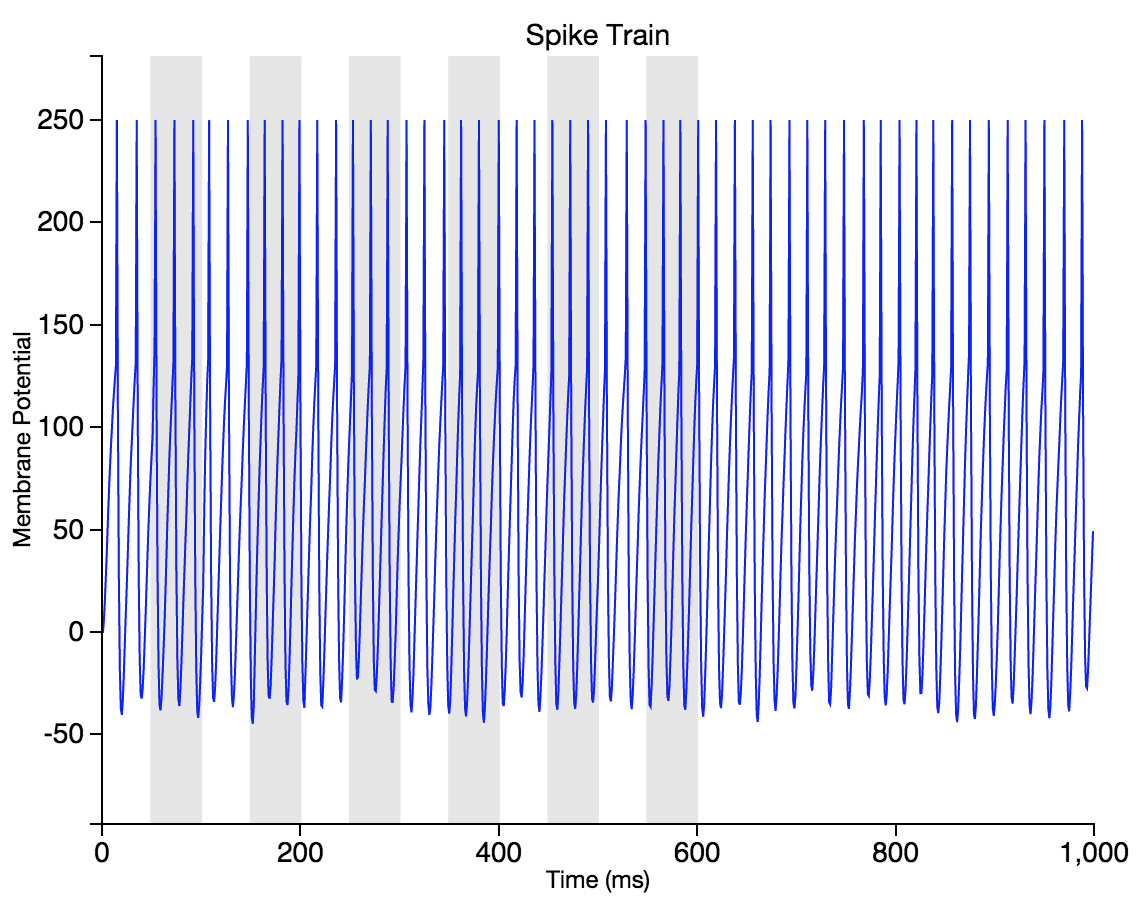
\includegraphics[scale = 0.3]{single_pattern_beginning}
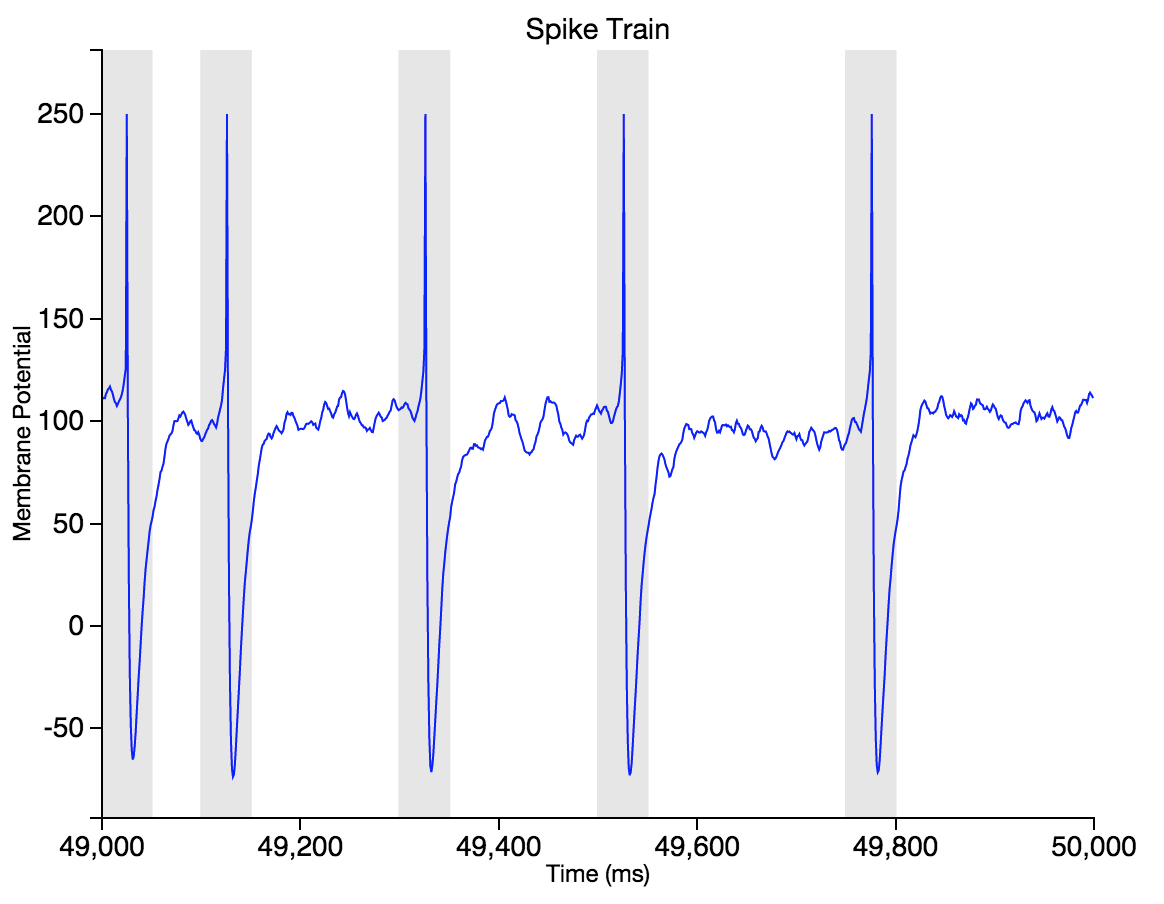
\includegraphics[scale = 0.3]{single_pattern_end} \\
\end{figure}

\newpage

\subsection{Multiple Neurons / Multiple Patterns}
A network of mutually-inhibiting pattern recognition neurons are able to detect multiple patterns (shown in various colours) within a noisy background. As with the single neuron, at the beginning of the simulation the neurons fire a lot, as shown below on the left. However, towards the end some neurons become selective to multiple patterns and others, inhibited by their counterparts, cease to fire, as shown below on the right.

\begin{figure}[h]
\centering
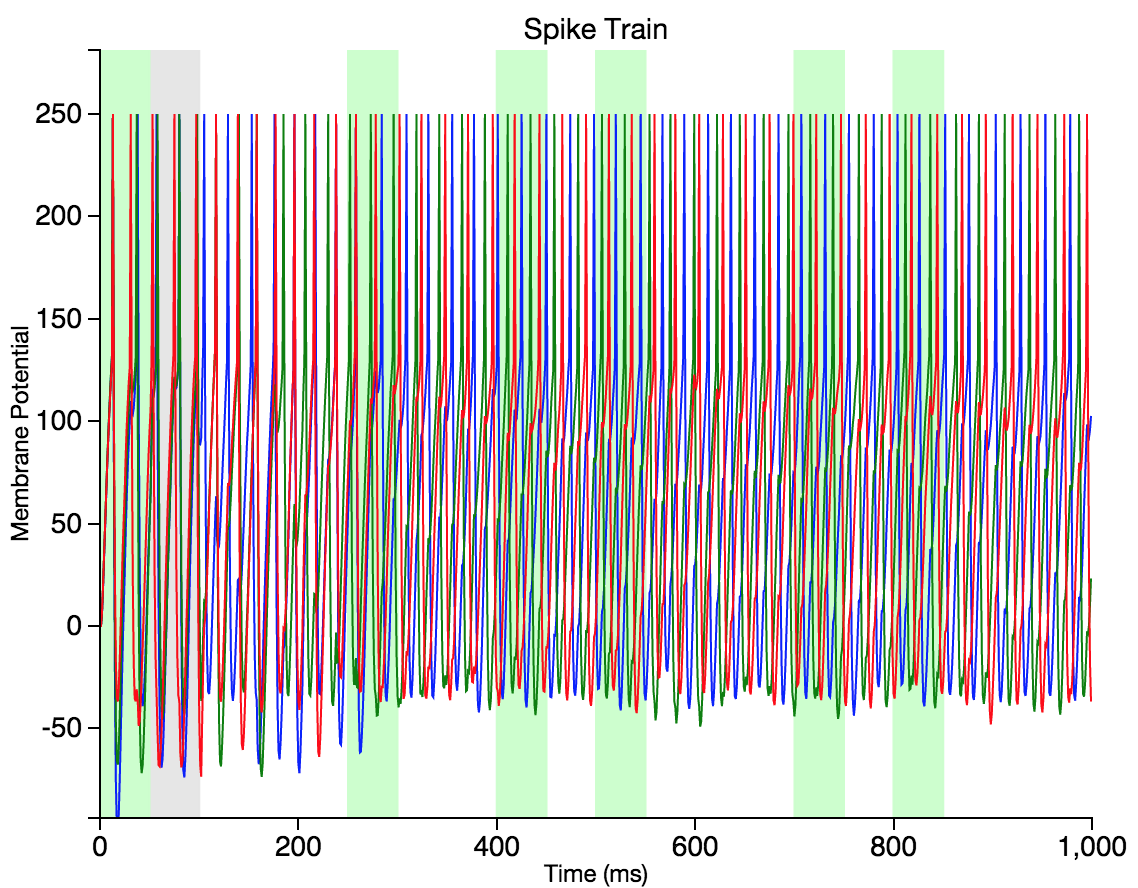
\includegraphics[scale = 0.3]{multiple_beginning}
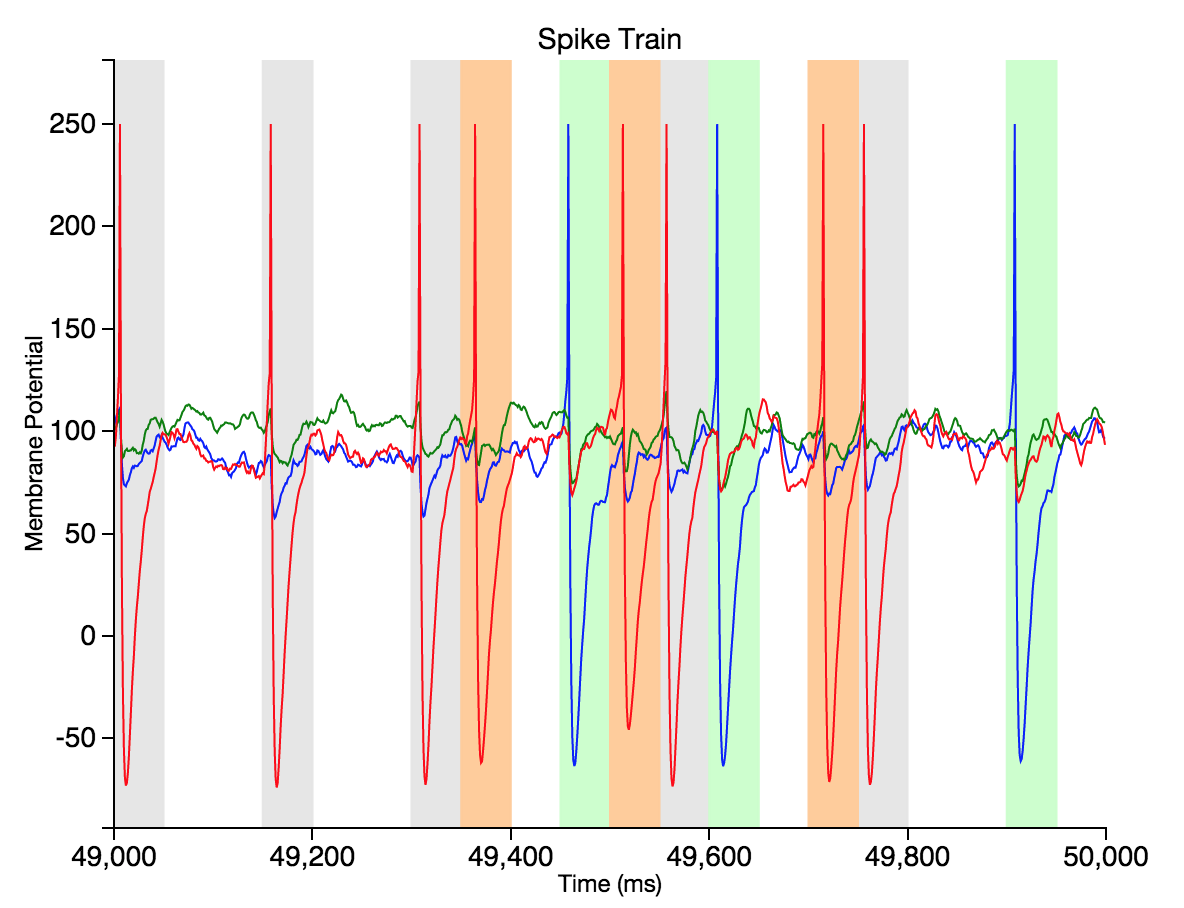
\includegraphics[scale = 0.3]{multiple_end}
\end{figure}

\section{Test Results}

\subsection{Overview}
\begin{minted}{bash}
$ coverage report -m

Name 		Stmts    Miss    Branch    BrMiss    Cover    Missing
------------------------------------------------------------------------------------------
estmd                 114      0        16        1        99%   
cstmd                 380      84       130       44       75%     213, 218, 317-401,
                                                                   487-488, 513-514,
                                                                   600-603, 638,
                                                                   642, 647-648, 662
target_animation      125      0        20        1        99%   
neuron                248      59       72        32       72%     170-179, 197, 209-212,
                                                                   216, 230-233, 237, 261,
                                                                   300, 331, 357, 368-381,
                                                                   388-393, 417-420,
                                                                   447-450, 488, 562-563,
                                                                   570-579
sample                127      0        32        0       100%   
simulation            109      35       30        18       62%     88-103, 133, 144-146,
                                                                   159-162, 175, 202-232
sample_dao            52       8        10        2        84%     78, 113-120
server                80       19       6         3        74%     44-51, 59, 79, 93-100,
                                                                   146, 160-161
simulation_dao        154      18       46        14       84%     34-35, 88, 118, 160-161,
                                                                   239-247, 259-260, 285
------------------------------------------------------------------------------------------
TOTAL                 1389     223      362       115      81%  
\end{minted}

\subsection{Individual Tests}
\subsubsection{Visual Pre-processing Module}
\subsubsection*{ESTMD}
\begin{minted}{bash}
$ coverage run --branch test_estmd.py
....
----------------------------------------------------------------------
Ran 4 tests in 3.845s

OK
\end{minted}
\subsubsection*{Target Animation}
\begin{minted}{bash}
$ coverage run --branch test_target_animation.py
...........
----------------------------------------------------------------------
Ran 11 tests in 2.615s

OK
\end{minted}

\subsubsection{Dragonfly Neuron Module}
\subsubsection*{CSTMD}
\begin{minted}{bash}
$ coverage run --branch test_cstmd.py
..
----------------------------------------------------------------------
Ran 3 tests in 64.135s

OK
\end{minted}

\subsubsection{Pattern Recognition Module}
\subsubsection*{Neuron}
\begin{minted}{bash}
$ coverage run --branch test_neuron.py
................
----------------------------------------------------------------------
Ran 16 tests in 0.197s

OK
\end{minted}

\subsubsection*{Sample}
\begin{minted}{bash}
$ coverage run --branch test_sample.py
.
----------------------------------------------------------------------
Ran 6 tests in 39.788s

OK
\end{minted}

\subsubsection*{Simulation}
\begin{minted}{bash}
$ coverage run --branch test_simulation.py
..
----------------------------------------------------------------------
Ran 2 tests in 1.080s

OK
\end{minted}

\subsubsection{Web Client Module}
\subsubsection*{Sample Data Access Object}
\begin{minted}{bash}
$ coverage run --branch test_sample_dao.py 
.
----------------------------------------------------------------------
Ran 1 test in 7.838s

OK
\end{minted}

\subsubsection*{Server}
\begin{minted}{bash}
$ coverage run --branch test_server.py
...
----------------------------------------------------------------------
Ran 8 tests in 5.172s

OK
\end{minted}

\subsubsection*{Simulation Data Access Object}
\begin{minted}{bash}
$ coverage run --branch test_simulation_dao.py
----------------------------------------------------------------------
Ran 1 test in 5.211s

OK
\end{minted}

\end{appendices}




\end{document}

